%!TEX TS-program = xelatex

\documentclass[c, dvipsnames]{beamer}  % [t], [c], или [b] --- вертикальное
%\documentclass[handout, dvipsnames, c]{beamer} % Раздаточный материал (на слайдах всё сразу)



%%%%%%%%%% Работа с картинками %%%%%%%%%
\usepackage{graphicx}                  % Для вставки рисунков
\usepackage{graphics}
\graphicspath{{images/}{pictures/}}    % можно указать папки с картинками
\usepackage{wrapfig}                   % Обтекание рисунков и таблиц текстом


%%%%%%%%%% Работа с таблицами %%%%%%%%%%
\usepackage{tabularx}            % новые типы колонок
\usepackage{tabulary}            % и ещё новые типы колонок
\usepackage{array}               % Дополнительная работа с таблицами
\usepackage{longtable}           % Длинные таблицы
\usepackage{multirow}            % Слияние строк в таблице
\usepackage{float}               % возможность позиционировать объекты в нужном месте
\usepackage{booktabs}            % таблицы как в книгах!
\renewcommand{\arraystretch}{1.3} % больше расстояние между строками

\usepackage{pgf,tikz}
\usepackage{mathrsfs}
\usetikzlibrary{arrows}


%выравнивание на слайдах (верх, центр, низ)
%\documentclass[handout, dvipsnames]{beamer} % Раздаточный материал (на слайдах всё сразу)
%\documentclass[aspectratio=169, dvipsnames]{beamer} % Соотношение сторон
\setbeamertemplate{navigation symbols}{}%remove navigation symbols

%\usetheme{Berkeley} % Тема оформленияLLL
%\usetheme{Bergen}
%\usetheme{CambridgeUS}
\usetheme{Boadilla}

\usecolortheme{crane} % Цветовая схема

%\useoutertheme{infolines} % Навигация 
%\useoutertheme{tree}
%\useoutertheme{miniframes}
%\useoutertheme{shadow}
%\useoutertheme{sidebar}
%\useoutertheme{smoothbars}
%\useoutertheme{smoothtree}
%\useoutertheme{split}
%\useoutertheme{default}


%\useinnertheme{circles}
\useinnertheme{rectangles}
%\useinnertheme{rounded}
%\useinnertheme{inmargin}


%%% Работа с русским языком
\usepackage[english,russian]{babel}   %% загружает пакет многоязыковой вёрстки
\usepackage{fontspec}      %% подготавливает загрузку шрифтов Open Type, True Type и др.
\defaultfontfeatures{Ligatures={TeX},Renderer=Basic}  %% свойства шрифтов по умолчанию
\setmainfont[Ligatures={TeX,Historic}]{Arial} %% задаёт основной шрифт документа
\setsansfont{Arial}                    %% задаёт шрифт без засечек
\setmonofont{Arial}
\usepackage{indentfirst}
\frenchspacing



%% Beamer по-русски
\newtheorem{rtheorem}{Теорема}
\newtheorem{rproof}{Доказательство}
\newtheorem{rexample}{Пример}

%%% Дополнительная работа с математикой
\usepackage{amsmath,amsfonts,amssymb,amsthm,mathtools} % AMS
\usepackage{icomma} % "Умная" запятая: $0,2$ --- число, $0, 2$ --- перечисление

%% Номера формул
\mathtoolsset{showonlyrefs=true} % Показывать номера только у тех формул, на которые есть \eqref{} в тексте.
%\usepackage{leqno} % Нумерация формул слева

%% Свои команды
\DeclareMathOperator{\sgn}{\mathop{sgn}}

%% Перенос знаков в формулах (по Львовскому)
\newcommand*{\hm}[1]{#1\nobreak\discretionary{}
{\hbox{$\mathsurround=0pt #1$}}{}}

%%% Работа с картинками
\usepackage{graphicx}  % Для вставки рисунков
\graphicspath{{images/}{images2/}}  % папки с картинками
\setlength\fboxsep{3pt} % Отступ рамки \fbox{} от рисунка
\setlength\fboxrule{1pt} % Толщина линий рамки \fbox{}
\usepackage{wrapfig} % Обтекание рисунков текстом

%%% Работа с таблицами
\usepackage{array,tabularx,tabulary,booktabs} % Дополнительная работа с таблицами
\usepackage{longtable}  % Длинные таблицы
\usepackage{multirow} % Слияние строк в таблице

%%% Программирование
\usepackage{etoolbox} % логические операторы

%%% Другие пакеты
\usepackage{lastpage} % Узнать, сколько всего страниц в документе.
%\usepackage{soul} % Модификаторы начертания
\usepackage{csquotes} % Еще инструменты для ссылок
\usepackage{multicol} % Несколько колонок


\usepackage{hyperref}
\usepackage{xcolor}
\hypersetup{        % Гиперссылки
    unicode=true,           % русские буквы в раздела PDF
    pdftitle={Заголовок},   % Заголовок
    pdfauthor={Автор},      % Автор
    pdfsubject={Тема},      % Тема
    pdfcreator={Создатель}, % Создатель
    pdfproducer={Производитель}, % Производитель
    pdfkeywords={keyword1} {key2} {key3}, % Ключевые слова
    colorlinks=true,        % false: ссылки в рамках; true: цветные ссылки
    linkcolor=,          % внутренние ссылки
    citecolor=green,        % на библиографию
    filecolor=magenta,      % на файлы
    urlcolor=blue           % на URL
} 

\usepackage{dcolumn}

%fffff3
\definecolor{backgr}{RGB}{146,26,29}
\definecolor{backgr1}{RGB}{230,43,37}
\definecolor{ex1}{RGB}{231,142,36}
\definecolor{ex2}{RGB}{249,155,28}
\definecolor{ex3}{RGB}{242,103,36}

\definecolor{red}{RGB}{230,43,37}
%\setbeamercolor{normal text}{fg=black,bg=backgr}
\setbeamercolor{frametitle}{bg=backgr,fg=white}
%\setbeamercolor{footline}{bg=backgr,fg=white}
%\setbeamercolor{normal text}{bg=yellow}
%\setbeamercolor{section in toc}{fg=yellow}
%\setbeamercolor{subsection in toc}{fg=blue}

% How to change colour of Navigation Bar in Beamer -  много интересного

%Пример команд, задающих внешний вид блока
\setbeamercolor{block title}{fg=white,bg=ex1}
\setbeamerfont{block title}{family=\sffamily}
\setbeamercolor{block body}{bg=white}
\setbeamertemplate{blocks}[rounded][shadow=fasle]
\setbeamercolor{title}{bg=backgr, fg=white}
\setbeamercolor{alerted text}{fg=backgr1}

\newlength\subtitwd
\setlength\subtitwd{4cm}% change the width here

\makeatletter
\newcommand\titlegraphicii[1]{\def\inserttitlegraphicii{#1}}
\titlegraphicii{}
\newcommand\superviser[1]{\def\insertsuperviser{Научный руководитель: #1}}
\superviser{}

\setbeamertemplate{title page}
{
  \vbox{}
   {\usebeamercolor[fg]{titlegraphic} \hspace{0.35ex} \inserttitlegraphic\hfill\inserttitlegraphicii \hspace{1ex} \par }\vspace{1.5ex}
  \begin{centering}
    \begin{beamercolorbox}[sep=8pt,center]{institute}
      \usebeamerfont{institute}\insertinstitute
    \end{beamercolorbox}
    \begin{beamercolorbox}[sep=8pt,center]{title}
    
      \usebeamerfont{title}\inserttitle\par%
      \ifx  \insertsubtitle\@empty%
      \else%
        \vskip0.5em%
        {\usebeamerfont{subtitle}\usebeamercolor[fg]{subtitle}\insertsubtitle\par}%
      \fi%     
    \end{beamercolorbox}%
    \vskip1em\par
    \begin{beamercolorbox}[sep=5pt,center]{date}
      \usebeamerfont{date}\insertdate
    \end{beamercolorbox}%\vskip0.5em
    \begin{beamercolorbox}[sep=5pt,center]{author}
      \usebeamerfont{author}\insertauthor
    \end{beamercolorbox}
        \begin{beamercolorbox}[sep=4pt,center]{institute}
      \usebeamerfont{institute}\insertsuperviser
    \end{beamercolorbox}
  \end{centering}
  %\vfill
}
\makeatother

\setbeamercolor{item projected}{bg=ex3}
\setbeamertemplate{enumerate items}[default]

\setbeamercolor{palette primary}{bg=white}
\setbeamercolor{palette primary}{fg=black}
\setbeamercolor{palette secondary}{bg=white}
\setbeamercolor{palette secondary}{fg=black}
\setbeamercolor{palette tertiary}{bg=white}
\setbeamercolor{palette tertiary}{fg=black}

\setbeamercolor{itemize item}{fg=ex3}
\setbeamercolor{itemize subitem}{fg=ex2}
\setbeamercolor{itemize subsubitem}{fg=ex1}

\setbeamercolor{enumerate item}{fg=ex3}
\setbeamercolor{enumerate subitem}{bg=ex3}
\setbeamercolor{enumerate subsubitem}{bg=ex3}


\setbeamertemplate{itemize subitem}{$\Rightarrow$}
\setbeamertemplate{itemize item}{$\blacktriangleright$}



\usepackage{todo}
\newcolumntype{a}{>{\columncolor{red}}c}


\usefonttheme{professionalfonts}

\title[  ]{Анализ влияния информационного фона на \\ стоимость финансовых активов}
\subtitle{магистерская программа  <<Экономика и Финансы>>}


\author[Ульянкин Филипп]{\scriptsize Студент: Ульянкин Филипп Валерьевич \\ \smallskip \href{mailto:filfonul@gmail.com}{\nolinkurl{filfonul@gmail.com} }}

\superviser{к.э.н. Синельникова-Мурылёва Е.В.}


%\author[Имя автора]{Имя автора \\ \smallskip \scriptsize \href{mailto:author@ranepa.ru}{author@ranepa.ru} \\ \smallskip  \href{http://ranepa.ru}{http://ranepa.ru} }

\institute[РАНХиГС]{ \uppercase{
  Российская Академия Народного Хозяйства и  \\ Государственной Службы при Президенте Российской Федерации}}
\date{2 июля 2018 г.}


\titlegraphic{
\includegraphics[scale=0.5]{logo1}}
\titlegraphicii{
\includegraphics[scale=0.6]{logo3}}



\usepackage{color, colortbl}


\begin{document}

\frame[plain]{\titlepage}	% Титульный слайд



\begin{frame}[c]{Актуальность исследования}

\begin{itemize}
%	\item  Поведенческая экономика: людское мышление нерационально (стадо, фрейминг, уверенность);
%	\item  Обмен информацией, принятие решение внутри  информационно фона;
%	\item  Укрепление бумаги $\Rightarrow$ позитивные новости $\Rightarrow$ укрепление бумаги;
%	\item  Общий эмоциональный окрас новостей вокруг бумаги --- информационный фон;
%	\item  Оркаска фона влияет на решения инвесторов $\Rightarrow$ влияет на котировки;
%	\item  Хочется знать какая окраска у информационного фона сейчас и как она меняется во времени.

%\item  Информационный фон --- это общий эмоциональный окрас новостей вокруг ценной бумаги;
%\item  Окраска фона влияет на решения инвесторов $\Rightarrow$ влияет на котировки;
%\item  Укрепление бумаги $\Rightarrow$ позитивные новости $\Rightarrow$ укрепление бумаги;
%\item  Зная текущее состоянее информационного фона можно предсказать движение котировок.

\item Каждый год объёмы неструктурированной текстовой информации растут; 
\item В последнее время интенсивно развиваются алгоритмы машинного обучения, позволяющие обрабатывать её;
\item Понимание общего фона новостей и записей в социальных сетях может помочь в объяснении динамики различных экономических переменных.

\end{itemize}
\end{frame}


\begin{frame}[c]
\frametitle{Анализ предметной области}
{ \scriptsize
	\begin{table}[]
		\centering
		\resizebox{\textwidth}{!}{
			\begin{tabular}{|p{2.2cm}|p{1.8cm}|p{3.5cm}|p{7cm}|}
				\hline\rowcolor{backgr}
				\textcolor{white}{Авторы} & \textcolor{white}{Выборка, период}  & \textcolor{white}{Метод исследования}& \textcolor{white}{Результат} \\
				\hline
				(Utaka, 2003)  & Япония, 04/1983 - 09/1998  &   ИФН на основе соц. опросов   & Индекс поиска грейнджер причина для потребления. AIC, BIC и RMSE выбирают расширенную модель.\\
				\hline
				(Varian and Choi, 2012 )  & CША, 01/2004 - 12/2011    &  Индекс поиска &   Индекс поиска улучшает прогнозы для рынка недвижимости, безработицы, позволяет прогнозировать индекс доверия потребителей. \\
				\hline
			   (Bloom, 2009)  & США, 01/1965 - 12/2009 & Индекс новостей  &   Индекс принимает высокие значения  перед различными знаковыми событиями.  \\
			   \hline
			   	(Curme et all, 2014) & США, 04/01/2004 - 16/01/2012  & Тематическое моделирования, индекс поиска & Увеличение объема поиска по политическим и экономическим темам предшествует падению рынка. Торговля на основе поиска даёт значимый доход. Прочность связи уменьшается. \\
			   \hline
			   (Yakovleva, 2017)   & Россия, 01/2014 - 01/2017   & Тематическое моделирование & Встречаемость тем в СМИ помогает предсказать PMI.  AIC, BIC и RMSE выбирают расширенную модель. \\
			   \hline
			   (Frisbee, 2010 ) & США, 10/07/2006 - 21/12/2009 &  Анализ тональности мнений в финансовых блогах & Объем торговли в большей степени зависит от общих рыночных условий (ставка по федеральным фондам), чем от настроений инвесторов.	\\			\hline
			   (Bollen, Mao and Zeng, 2011)   &  28/02/2008 - 19/12/2008  & Анализ тональностей Twitter &  Отношение позитивных твиттов к негативным, спокойные посты, счастливые посты грейнджер-причина для динамики индекса Доу-Джонса. Учёт эмоций улучшает прогнозы нейросети.\\
			   \hline
		\end{tabular} }
	\end{table}
}
\end{frame}


\begin{frame}[shrink=3]
\frametitle{Цели и задачи}
	\begin{block}{Цель:}
	\begin{itemize}
		% \item Подтверждение влияния информационного фона на формирование цен финансовых активов в России.
	    \item Проверить оказывает ли изменение информационного фона влияние на формирование цен финансовых активов в России.
	    
	\end{itemize}

	\end{block}

	 	\begin{block}{Задачи:}
			\begin{enumerate}
	\item Обобщить актуальные исследования по вопросу взаимосвязи информационного фона с котировками.
	\item Проанализировать методологии, используемые для анализа информационного фона.
	\item Выбрать методы машинного обучения и эконометрические методы для дальнейшего анализа.
	\item Собрать и провести предварительную обработку необходимых данных.
	\item Проверить работоспособность выбранных способов учёта информационного фона на российских данных. Сравнить их между собой.
	 \end{enumerate}
	\end{block}
\end{frame}



\begin{frame}[c]{Данные используемые в исследовании}
\begin{enumerate}
\item  Индекс РТС  (дневная и месячная динамика);
\item  Индекс финансовых настроений сбербанка (месячная динамика);
\item  Данные о динамике поисковых запросов из Google-trends  (месячная динамика);
\item  Новостные тексты из ряда интернет СМИ.
\end{enumerate}

\vfill

\begin{itemize}
	\item  Новости собраны за период с 1 января 2009 года по 31 декабря 2017 года (больше 1 млн. новостей, 200 тыс. экономических новостей).
\end{itemize}
\end{frame}


\begin{frame}{Первый этап исследовательской работы}
 \begin{center}
 	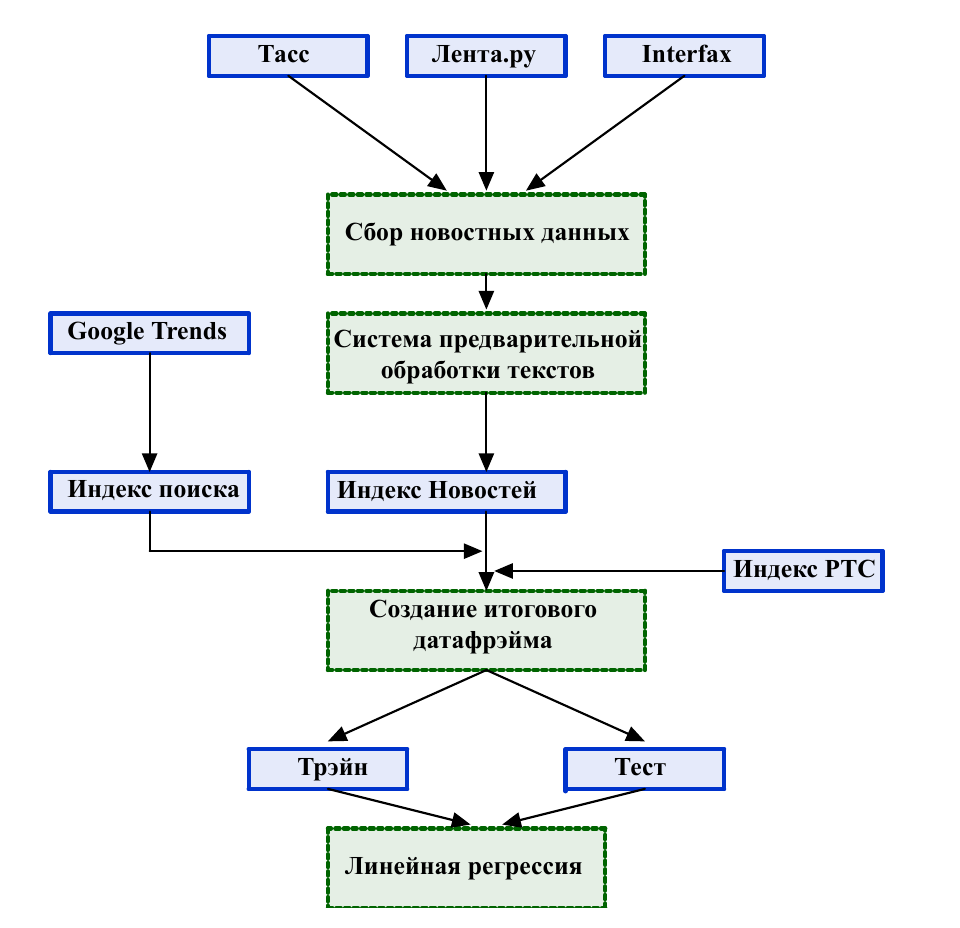
\includegraphics[width=0.7\textwidth]{etappp_1.png}
 \end{center}
 \end{frame}


\begin{frame}{Частотные индексы} 

	\begin{center}
			\scriptsize
	\begin{tabular}{llll}
		\toprule
		целевая переменная  &  причина &  p-значение  &   результат теста (5\%)  \\
		\midrule
		RTS d   &  ind IFN  &  0.336  & не является причиной по Грейнджеру \\ 
		ind IFN &  RTS d    &  0.663  & не является причиной по Грейнджеру \\
		RTS d   &  ind poisk& 0.005  & причина по Грейнджеру \\
		ind poisk& RTS d    & 0.114  & не является причиной по Грейнджеру \\
		RTS d   &  ind news & 0.008  & причина по Грейнджеру \\
		ind news&  RTS d    &0.038  & причина по Грейнджеру \\
		\bottomrule
	\end{tabular}

\hfill
\begin{columns}
\begin{column}{.28\linewidth}
	\includegraphics[scale=0.2]{corrindex.png}
\end{column}

\begin{column}{.68\linewidth}
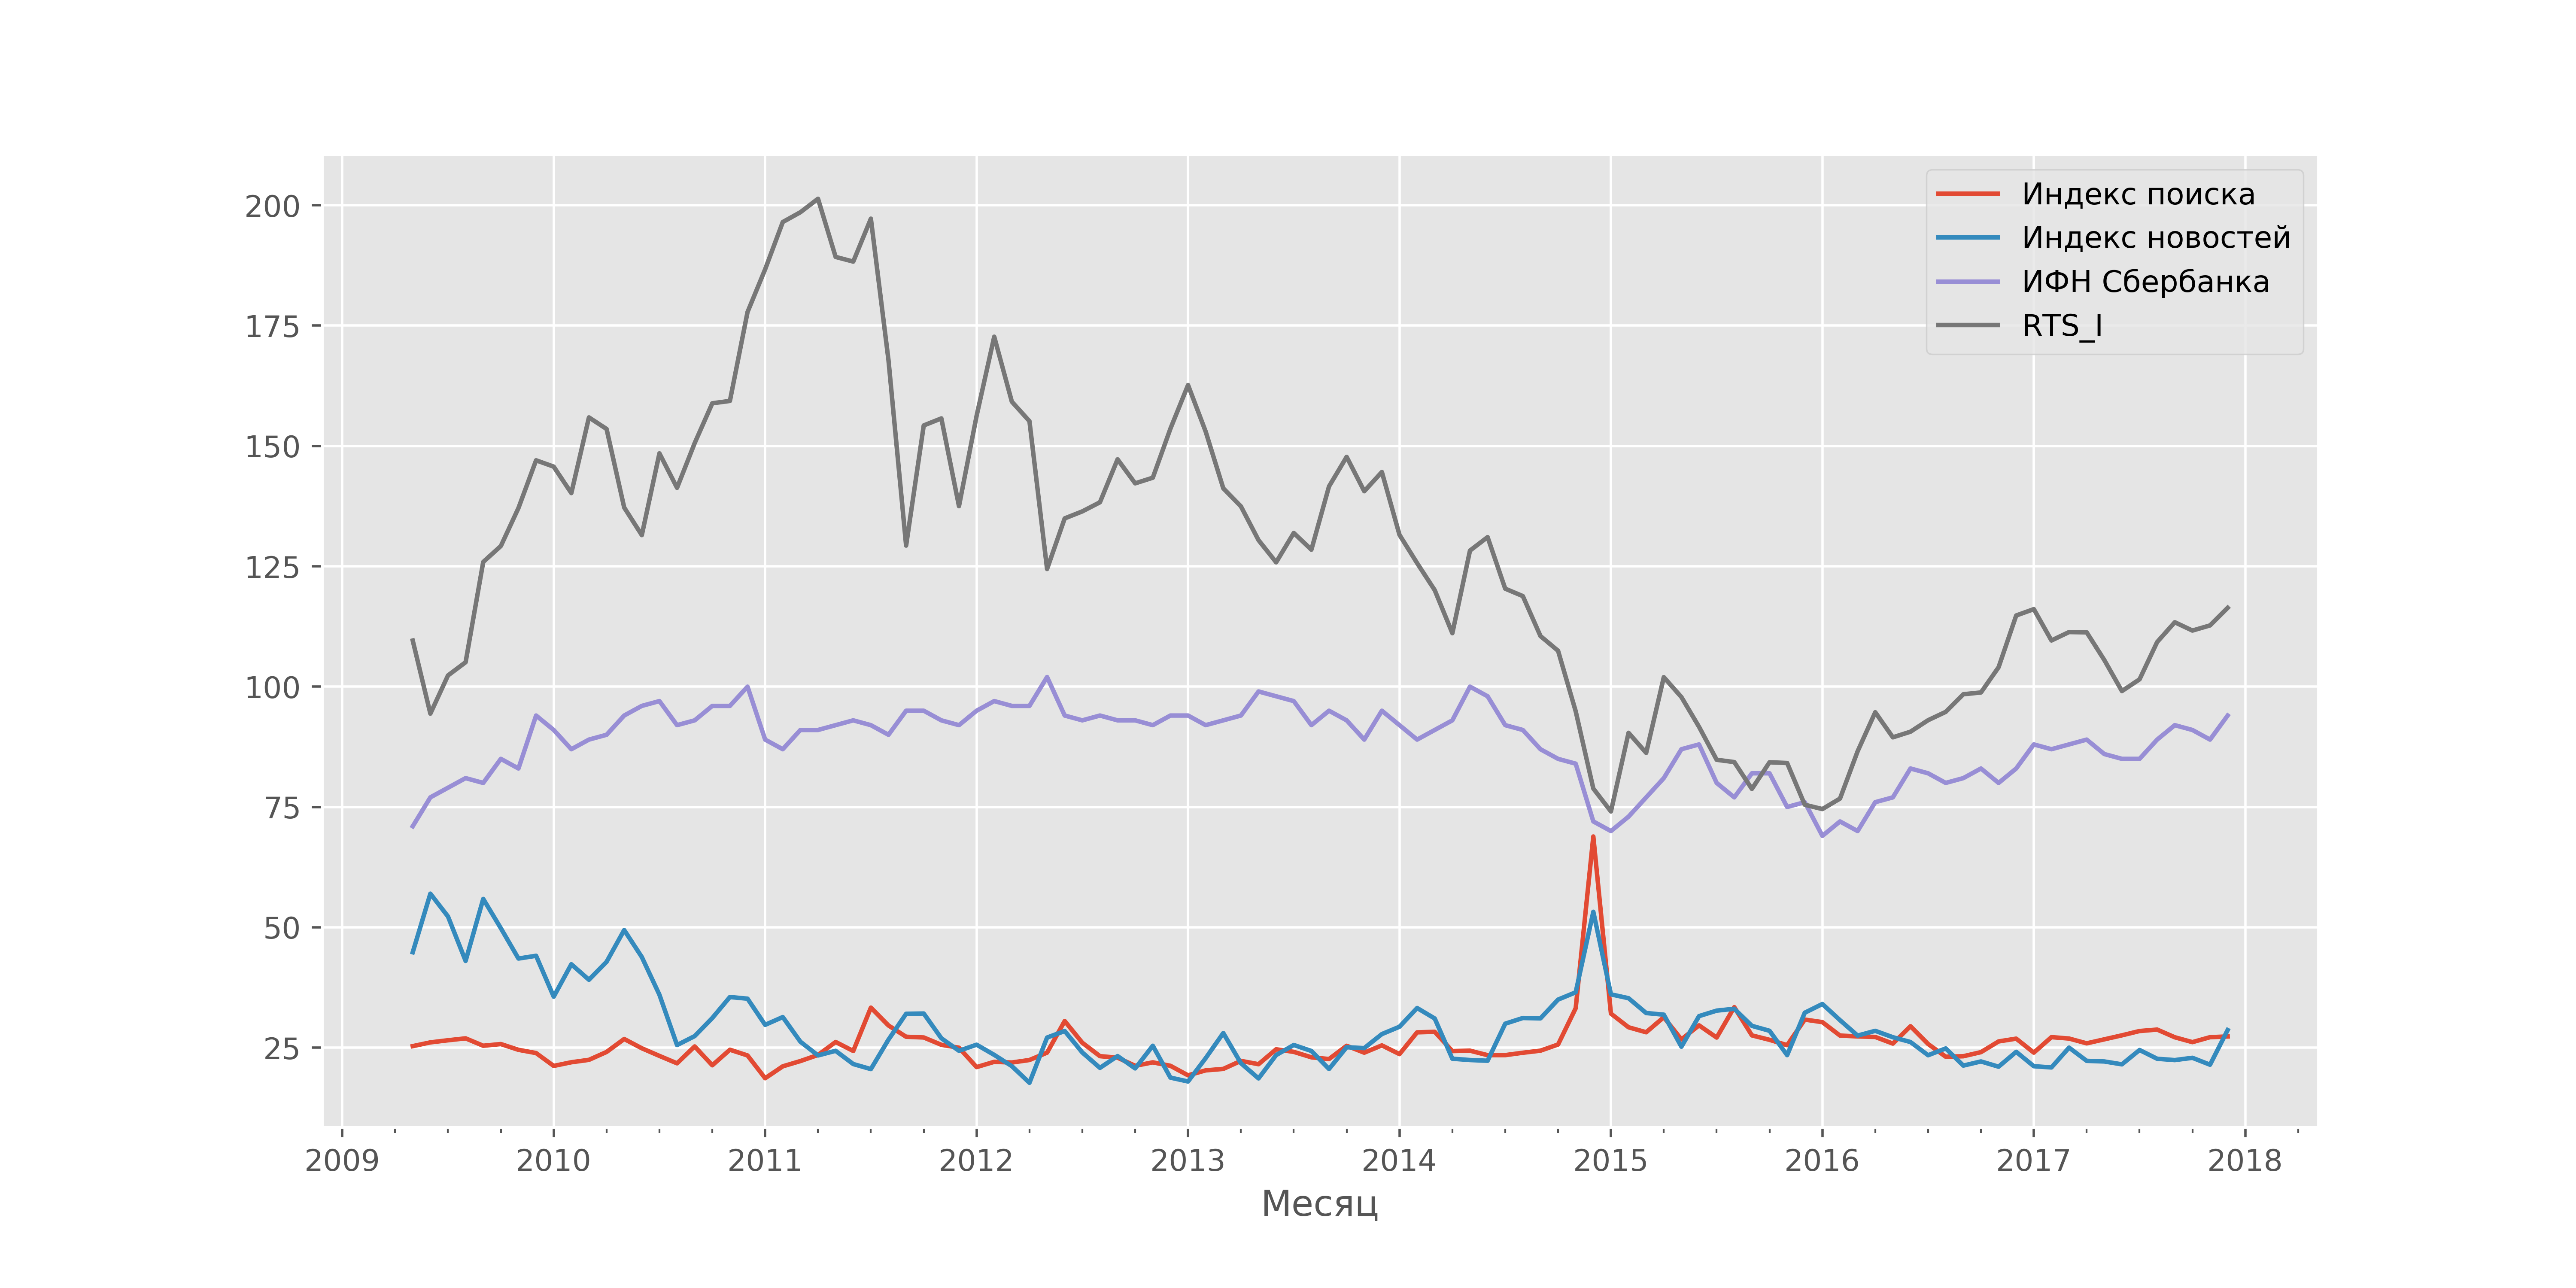
\includegraphics[scale=0.28]{allind.png}
\end{column}
\end{columns}
\end{center}
\end{frame}




 \begin{frame}{Частотные индексы}

\begin{center}
\scriptsize
\begin{tabular}{lcccc}
\hline
                                           & модель1                 &           модель 2        &    модель 3          &    модель 4 \\
\hline
$\Delta$  ind\_poisk      &  -0.005 (1.5e-3) *  &                                      &                                 &   -0.0042  (1e-3)* \\
$\Delta$  ind\_news      &                                    &    -0.004 (1.7e-3) *    &                                 &   -0.0008  (2e-3)\\
 $\Delta$ ind\_IFN         &                                    &                                       &   0.003 (2e-3)     &     0.0019  (2e-3) \\
 AIC  &   -172   &  -166 &   -164  &   -172  \\
 BIC  &   -167  &   -161  &  -159  &   -167  \\
 \hline
 \end{tabular}

\hfill

 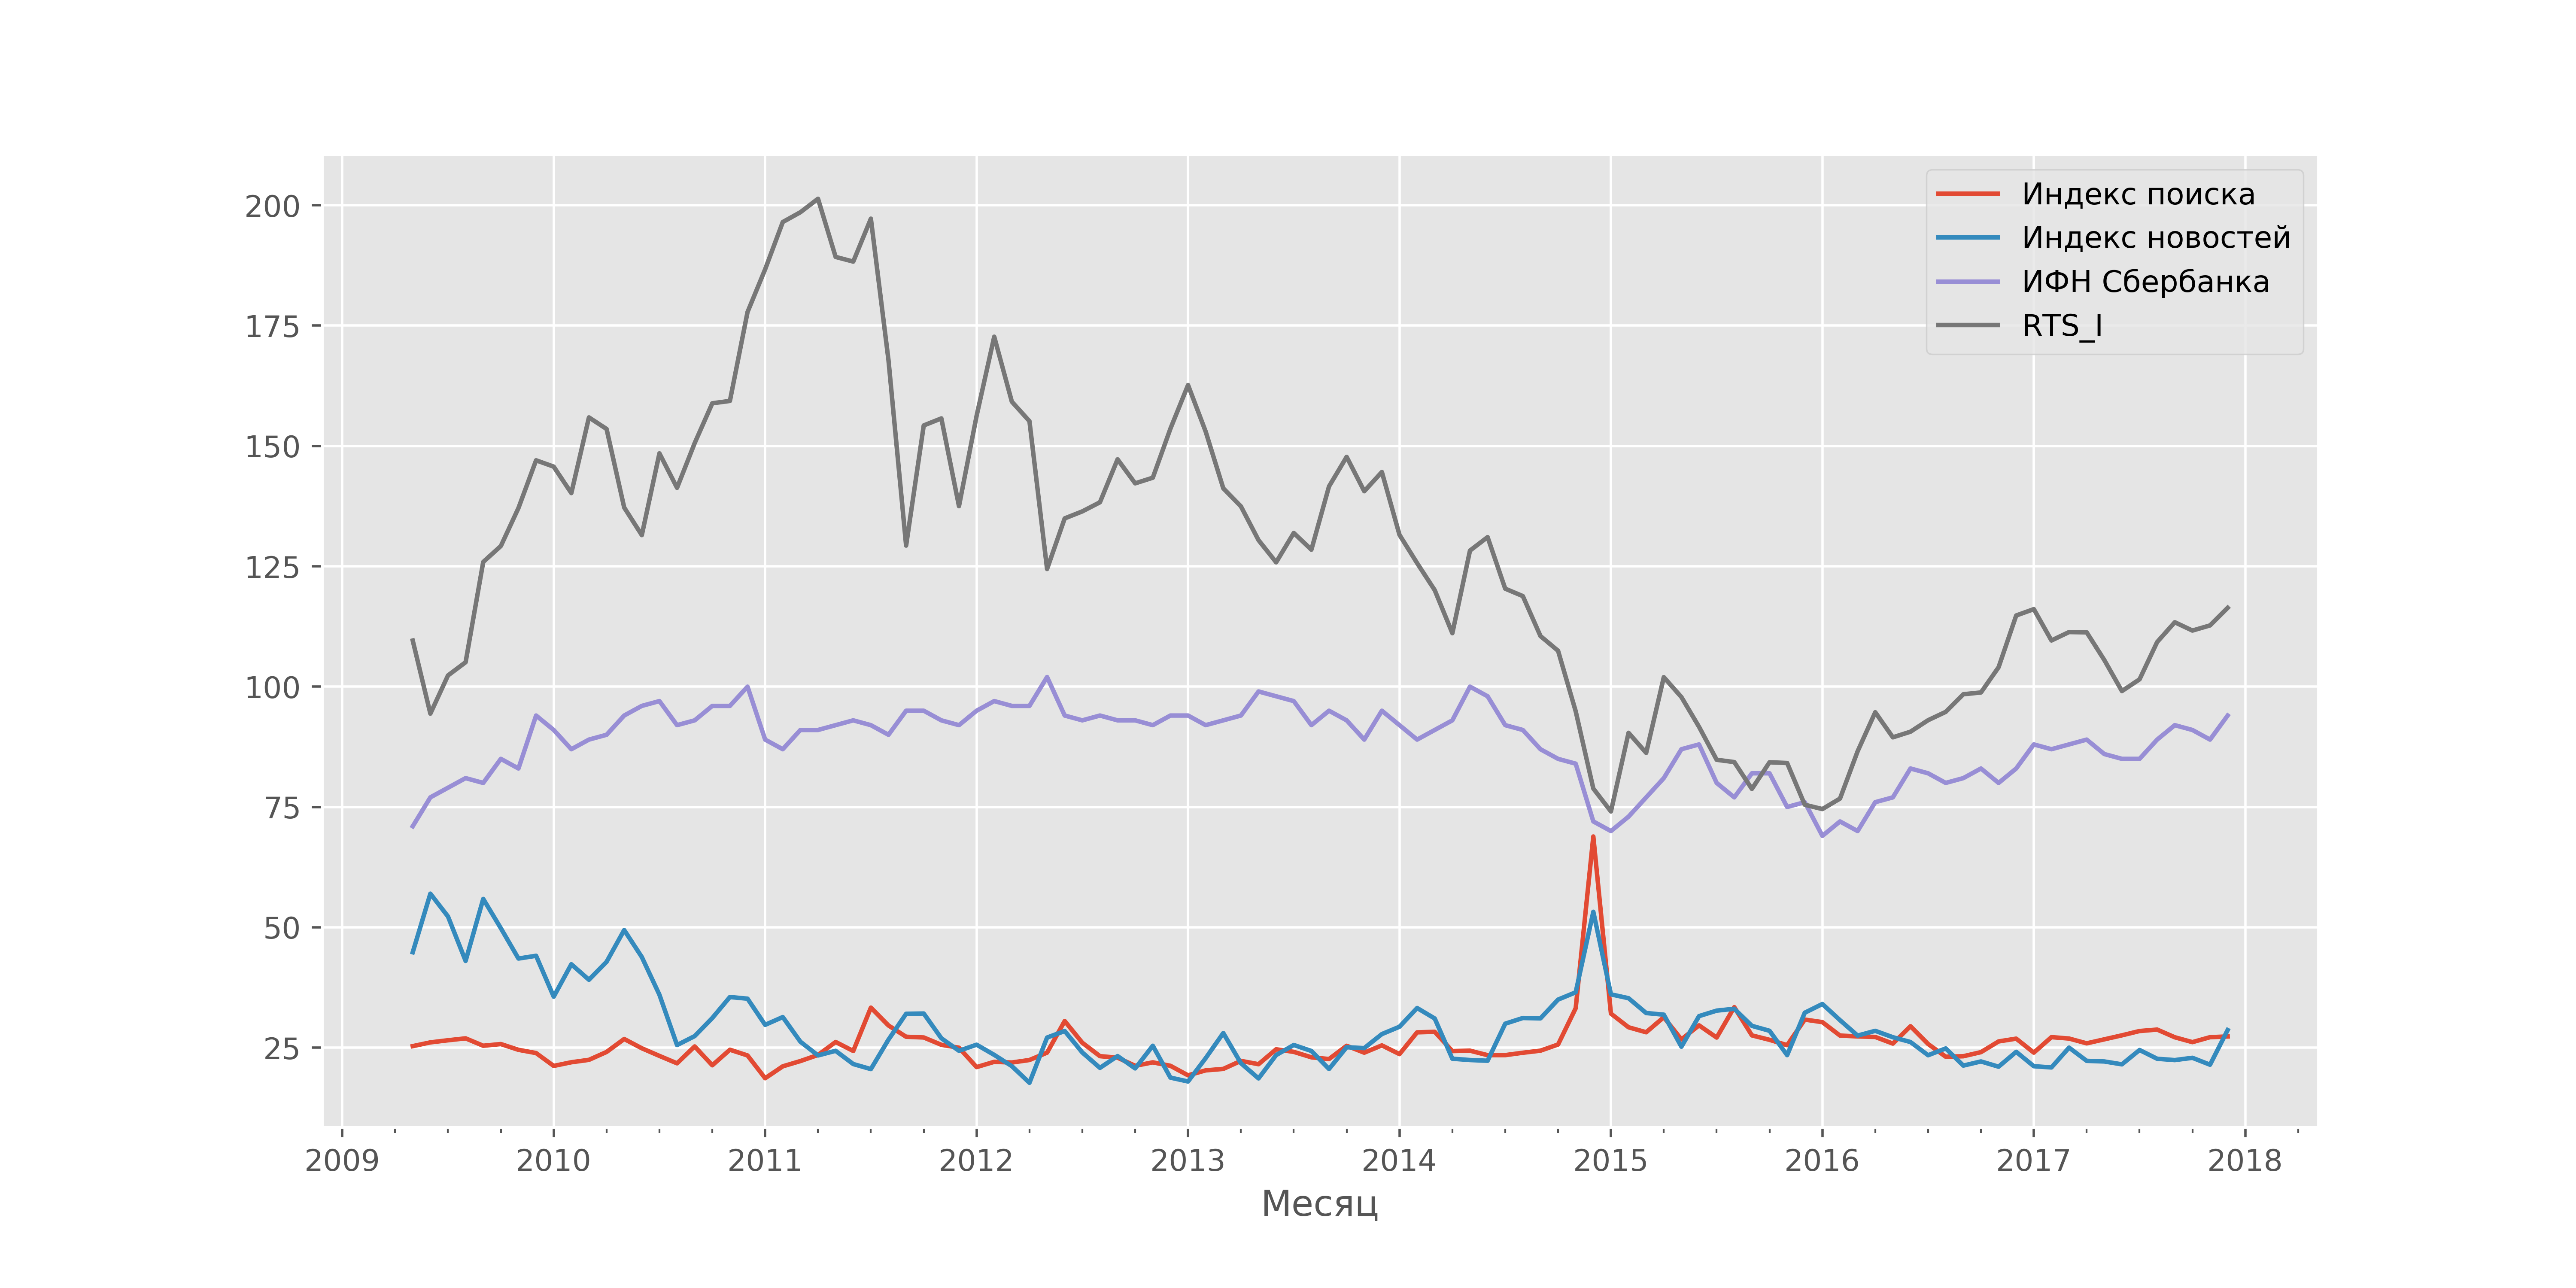
\includegraphics[scale=0.35]{allind.png}
\end{center}
\end{frame}



\begin{frame}{Второй этап исследовательской работы}
 \begin{center}
	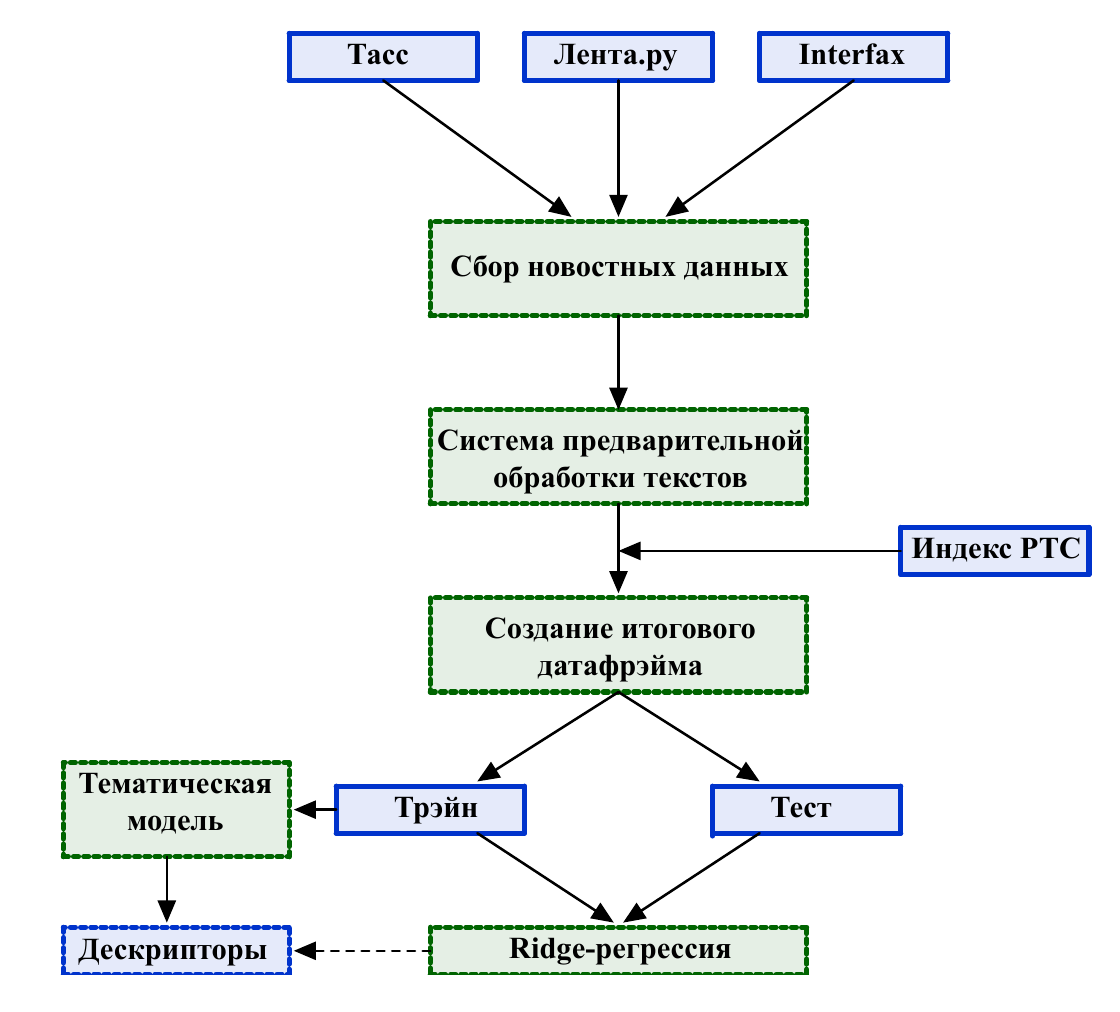
\includegraphics[width=0.69\textwidth]{etapp_2.png}
\end{center}
\end{frame}


\begin{frame}{Тематическое моделирование}
\begin{itemize}
	\item  Только экономические новости;
	\item  LDA-модель с 50 априорно заданными темами;
	\item Выборка: 01.01.2011 - 01.01.2017;
	\item  Oбъясняемые переменные: приросты тем за день.
\end{itemize}

\scriptsize
\begin{table}[ht]
	\centering
	\begin{tabular}{rrrrr}
		\hline
		& Estimate & Std. Error & t value & Pr($>$$|$t$|$) \\
		\hline
		X14 & 0.52  & 0.22  & 2.40 & 0.016 * \\
		X19 & -0.55 & 0.21 & -2.60 & 0.009** \\
		X20 & 0.37 & 0.11 & 3.18 & 0.001** \\
		X37 & -0.43 & 0.15 & -2.80 & 0.005** \\
		\hline
	\end{tabular}
\end{table}

\begin{block}{Интерпретация тем}
 	 Тема 14:  Западные страны,  \\ Тема 19:  Суды, следствия, \\ Тема 20: Поставки газа, газпром,  \\ Тема 37:  Страны ближнего востока и развивающиеся страны.
\end{block}
\end{frame}


\begin{frame}{Динамика индекса РТС и темы 19: суды, следствия }
 \begin{center}
	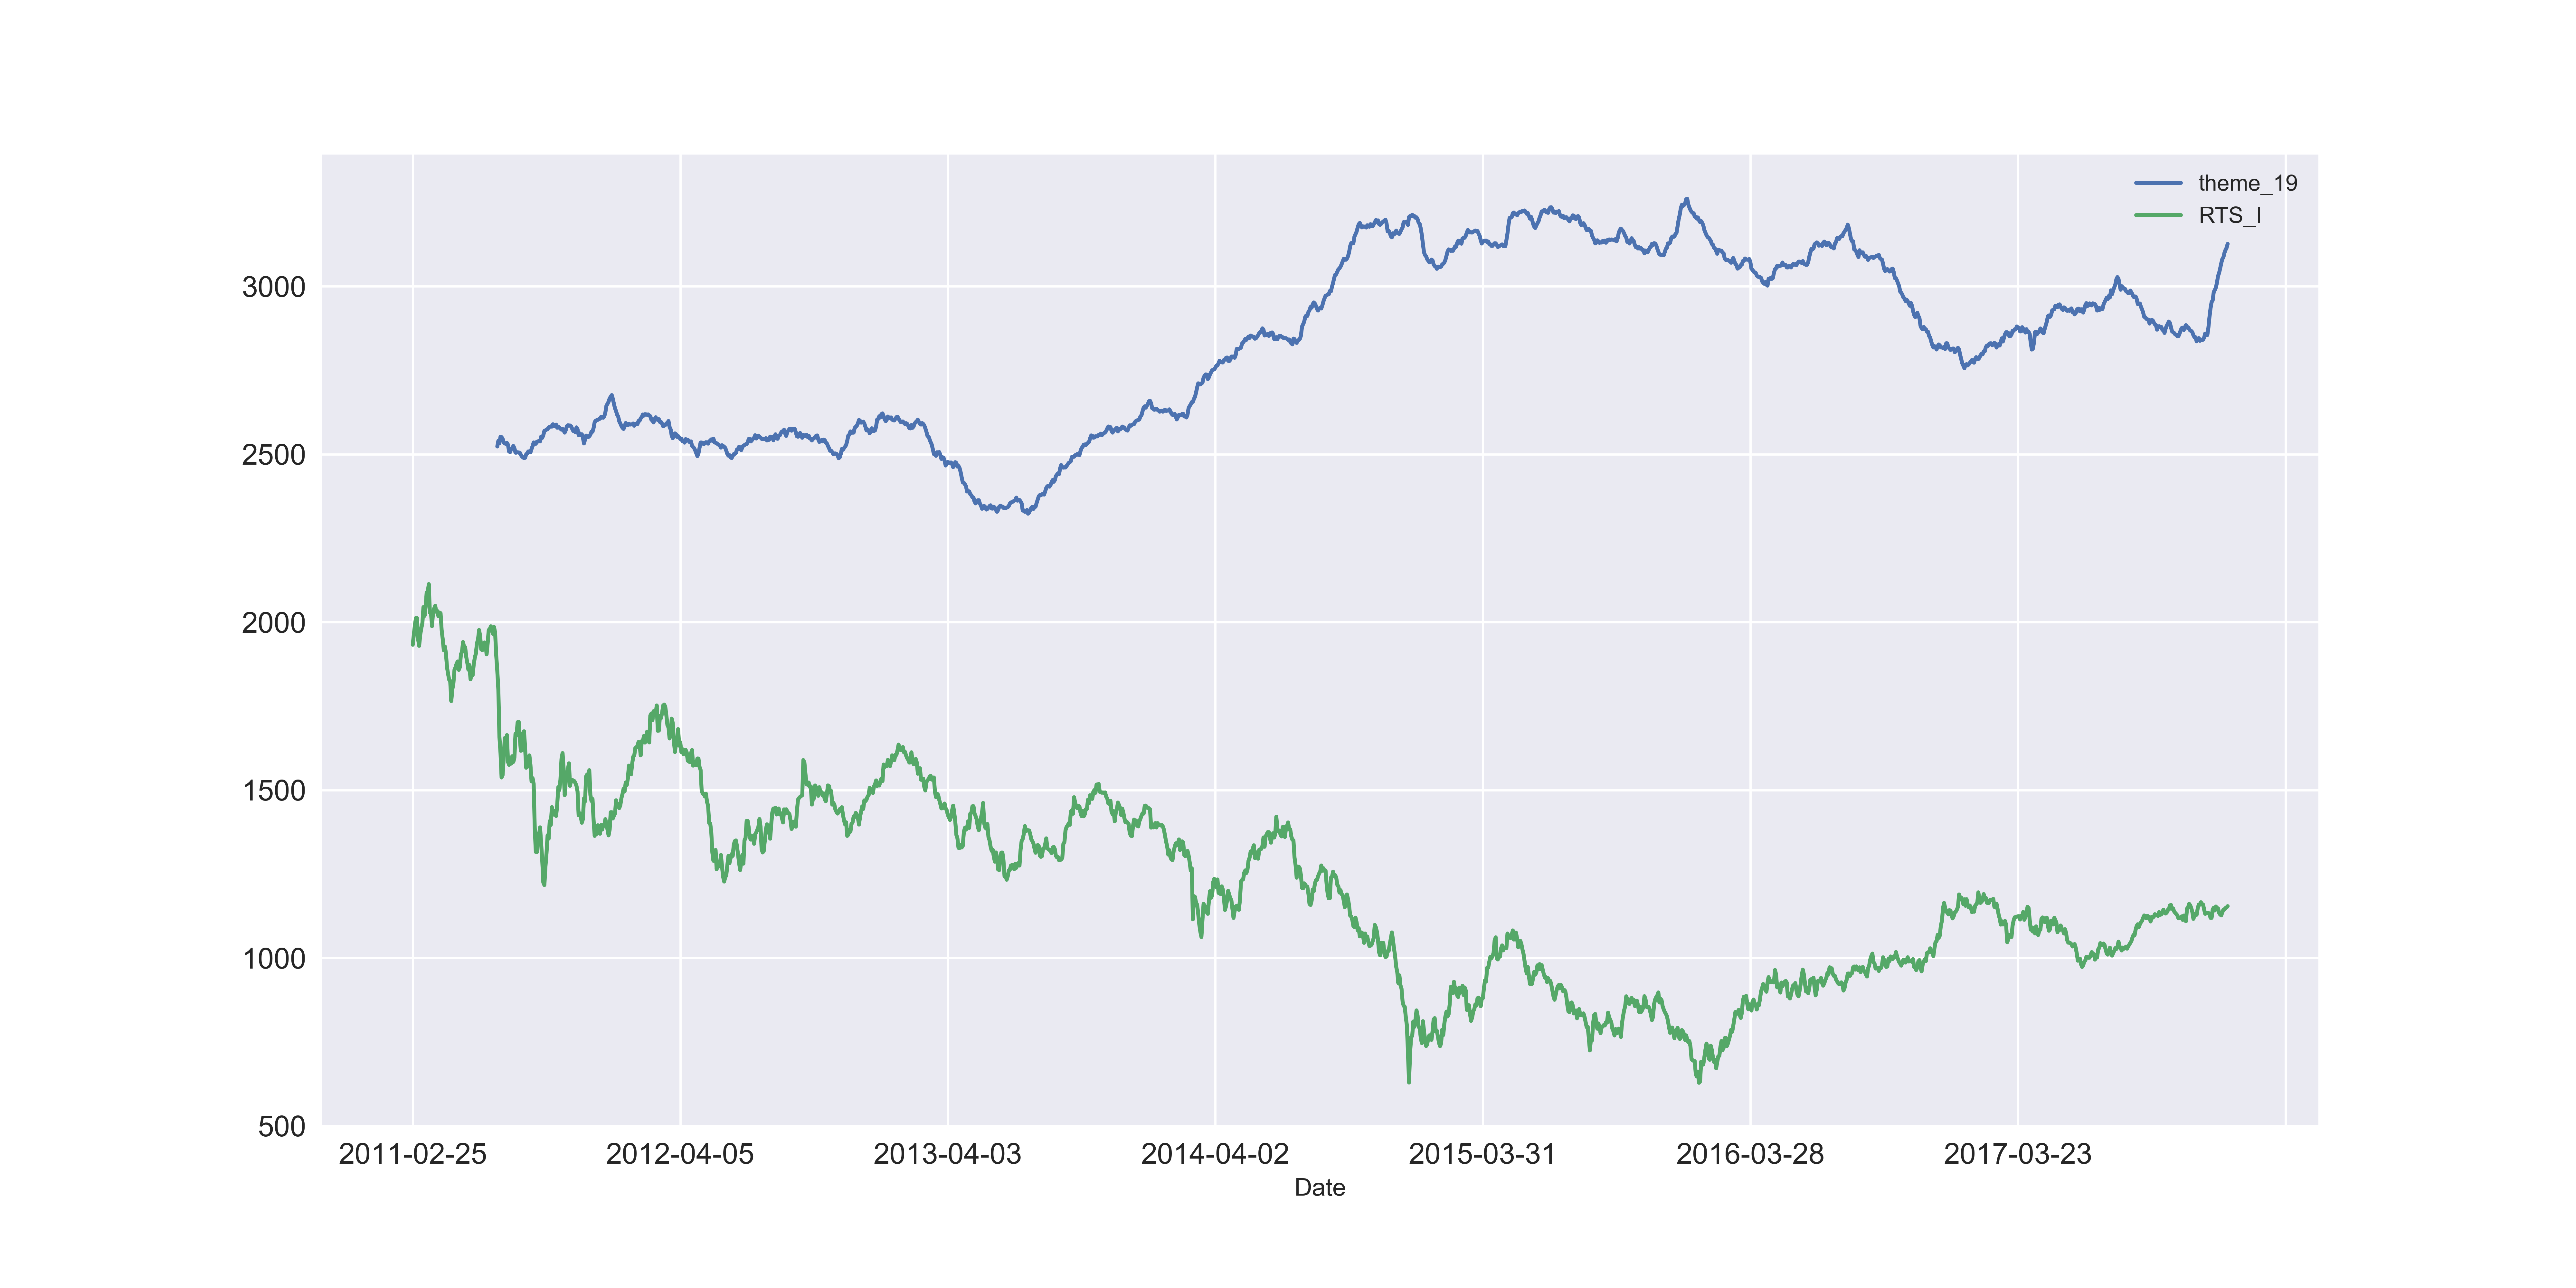
\includegraphics[scale=0.32]{dinamtheme_19.png}
\end{center}
\end{frame}



\begin{frame}{Ridge-регрессия}

\begin{itemize}
	\item   Экономические новости очищены от стоп-слов, токенизированы, лемматизированы, tf-idf;
	\item   Логистическая регрессия с $l_2$ регуляризатором;
	\item   Обучение модели:  SGD;
	\item  Train: 01.01.2014 - 01.01.2017;
	\item  Test:   01.01.2017 - 01.01.2018.
\end{itemize}


\begin{center}
{\scriptsize
\begin{tabular}{cccccc}
	\toprule
	Гиперпараметр $C$ &  Доходность  &  SR  & Просадка & 5\%  VaR  & Accuracy  \\
	\midrule
	$10^{-8}$	 &   -1.4\%  &  -1.3   &  18\% & 1.6\%  & 47.4\%   \\
	$10^{-5}	$ &   0.7\% &  0.6   &  20.4\%   &   1.7\%  &  51.4  \\
	$10^{-1}$	 &  24.1\%   &   22.7   & 11.5\%  &    1.6\%   & 51.4\%    \\
	%	$10^{0}$	 &  $-5.9\%$  &   $-4.7$  & $34.7\%$ &   $2.2\%$  &   $48.7\%$    \\
	$10^{1}$	 & \textbf{30.1\%}    &    \textbf{28.4}   &  \textbf{10.6\%}  &  1.6\%  &  \textbf{51.8\%}   \\
	$10^{5}$	 &  24.3\%  &   23  & 11.1\%  &  1.6\%  & 50.6\%    \\
	$10^{8}$	 &  27.5\% & 25.9    &  11.3\% &  1.6\%  &  51.4\%    \\
	\bottomrule
\end{tabular}
}
\end{center}
\end{frame}



\begin{frame}{Слова, формирующие фон}
\vspace{0.2cm}
\begin{columns}
	\begin{column}{.48\linewidth}
	    	{\tiny  \centering  $\qquad \quad $  Слова, формирующий положительный фон:} \\
	    	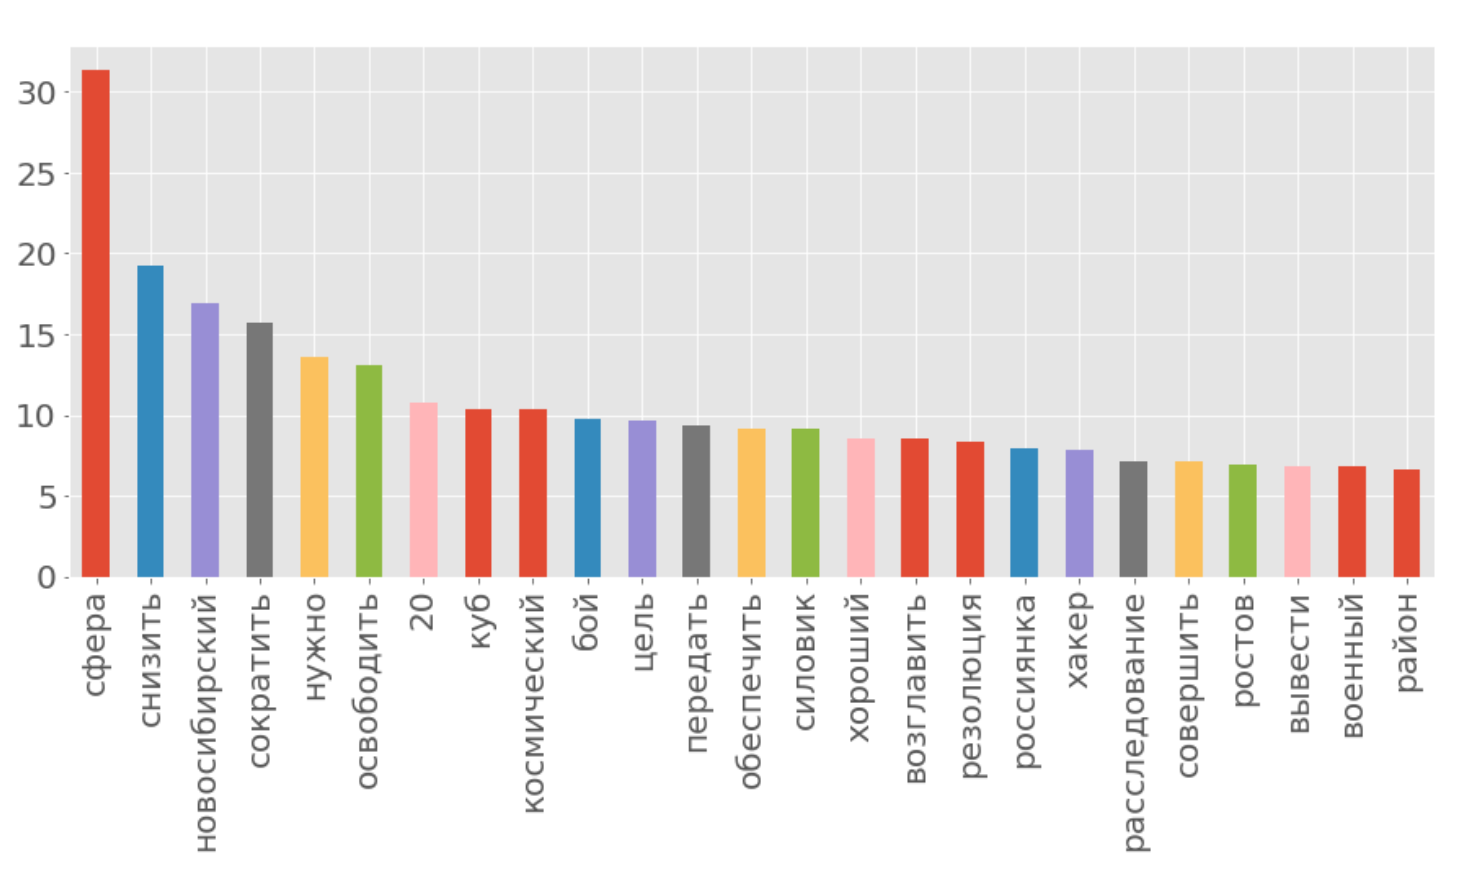
\includegraphics[width=0.99\textwidth]{top-word.png}
	\end{column}
	\begin{column}{.48\linewidth}
    	{\tiny \centering $\qquad \quad$ Слова, формирующий отрицательный фон: } \\
    	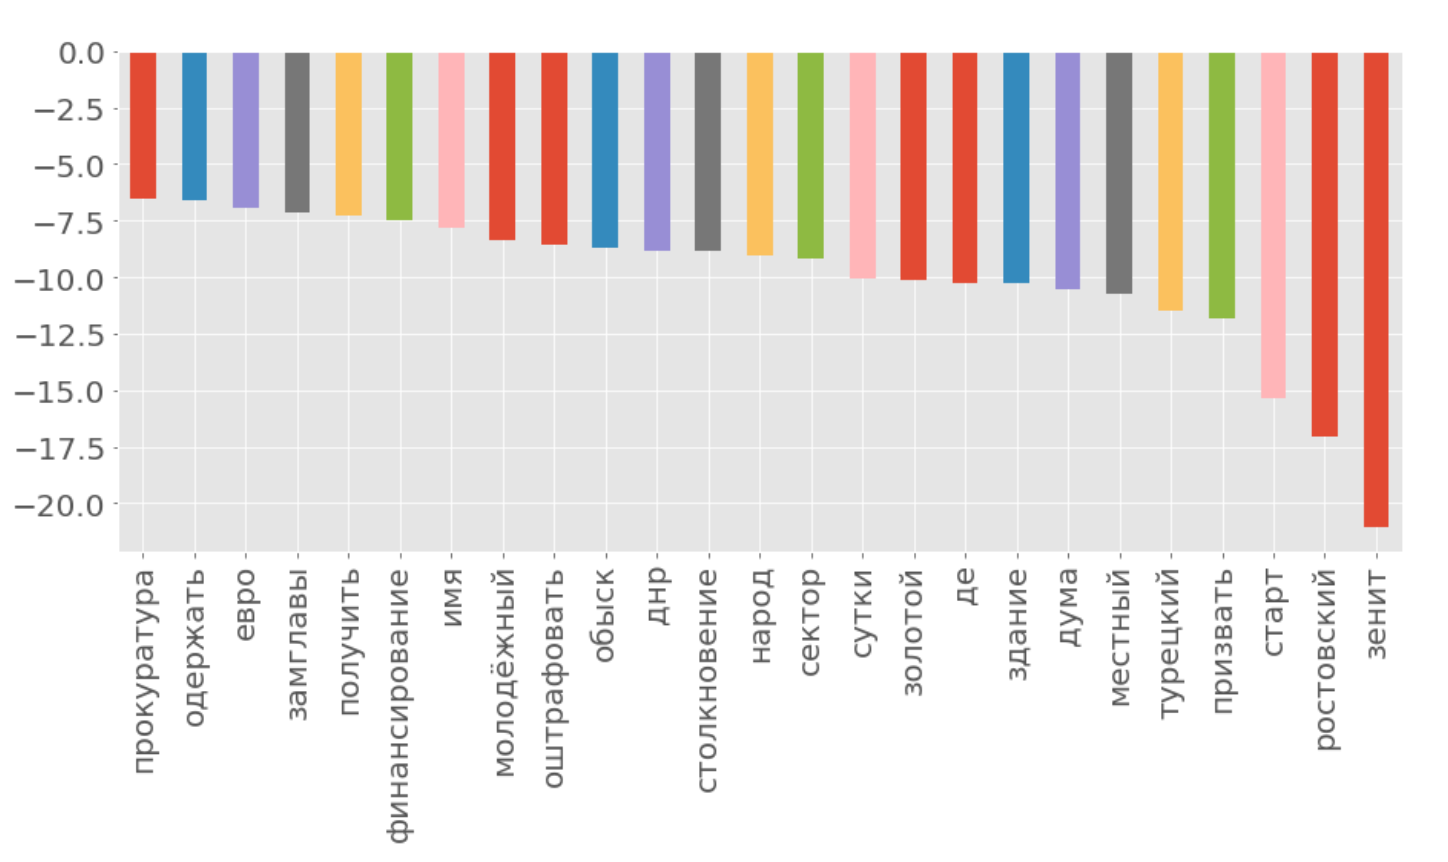
\includegraphics[width=0.99\textwidth]{bottom-word.png}
	\end{column}
\end{columns}

\begin{itemize}
\item Попытка использовать эти слова как дескрипторы для индекса новостей. Получена незначимая модель. 
\end{itemize}
\end{frame}


\begin{frame}{Теоретические результаты исследования}

\hspace{1.8cm}  {\color{ex1}  \textbf{Месячные данные:}}

\begin{center}
	{\scriptsize
		\begin{tabular}{lcccc}
	\toprule
	Модель  & AIC & SIC & MAPE   & RMSE    \\
	\midrule
	Наивный прогноз           & ---  & ---     & 3.77 & 0.052    \\
	Индекс поиска               & -172 & -167 &  1.17  &  0.051  \\
	Индекс новостей            & -166 & -161 & 2.32 & 0.052  \\  
	Индексы на основе Ridge& -134 & -127 &   3.98 &  0.062  \\ 
	\bottomrule
\end{tabular}
	}
\end{center}

\hspace{1.8cm}  {\color{ex1}  \textbf{Дневные данные:}}

\begin{center}
	{\scriptsize
\begin{tabular}{lcccc}
	\toprule
	Модель  & AIC & SIC & MAPE   & RMSE    \\
	\midrule
	Наивный прогноз           & ---       & ---        & 4.67 & 0.016  \\
	Индекс новостей            & -5914 & -5904  &  1.02 & 0.011   \\  
	Тематическая модель    & -6017 & -5991   & 1.78 &   0.012 \\
	Индексы на основе Ridge&  -5760   & -5744  & --- &  ---  \\
	Ridge-регрессия              & ---      & ---  & 1.22 & 0.010 \\
	\bottomrule
\end{tabular}
	}
\end{center}


\end{frame}


\begin{frame}{Практические результаты исследования}
\begin{itemize}
	\item  Разработаны индексы поиска, новостей, тематические индексы, позволяющие отслеживать динамику информационного фона;
	\item  Установлено, что новости, публикуемые в СМИ формируют информационный фон, оказывающий значимое влияние на индекс РТС;
	\item  Выявлено, что  значимое влияние на индекс РТС оказывают темы новостей, связанные с Западом, судом, поставками газа и странами ближнего Востока.
	\item  Найдены конкретные слова, появление которых в СМИ формирует положительный/отрицательный информационный фон.
\end{itemize}
\end{frame}



\begin{frame}[c, plain]
\begin{center}

{\LARGE Спасибо за внимание}

\bigskip

{\Large \inserttitle}

\bigskip

{\insertauthor}

\bigskip

\bigskip\bigskip

{\large \insertdate}
\end{center}
\end{frame}


%\section{Приложения}
%\begin{frame}[plain,c]
%\begin{center}
%\Huge{\textbf{
%	ПРИЛОЖЕНИЯ}}
%\end{center}
%
%\end{frame}




\end{document}
